Hier wird gezeigt wie ein Agent einen anderen verdrängt, aber auch das Agenten Umwege in Kauf nehmen.

\textbf{Aufbau des Experiments}
\begin{figure}[H]
    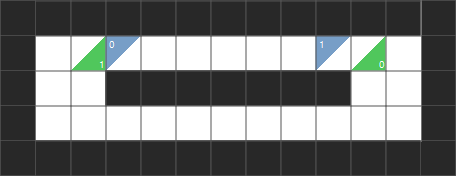
\includegraphics[height=40mm]{images/detour.png}
    \centering
    \caption{Aufbau für ein Szenario, in dem ein Agent einen Umweg in Kauf nimmt}
    \label{fig:umweg}
\end{figure}
Die Karte in Abbildung \ref{fig:umweg} misst elf mal drei Felder und wird mittig, horizontal durch einen Streifen aus sieben Feldern getrennt. Die Start- und Zielpositionen der Agenten sind so angeordnet, dass die nördliche Engstelle den kürzeren Weg darstellt und die südliche Engstelle den Umweg.

\textbf{Erwartete Beobachtungen}\newline
Für kleine Umgebungskarten, also solche bei denen sich die Umgebungskarten der beiden Agenten erst nach dem Annähern überlappen, werden sich beide Agenten in der nördlichen Engstelle annähern. Wenn sich die Umgebungskarten dann überlappen, wird einer der Agenten den Zuschlag erhalten und den anderen Agenten verdrängen. Dieser wird dann über die südliche Engstelle, also über den Umweg, sein Ziel anfahren.

Für größere Umgebungskarten wird der Agent, der zuerst seinen Weg plant, direkt und der andere über den Umweg sein Ziel anfahren.